\section{Mobile Traffic Classification}
\label{sec:classification-methodology}

\platname offers a network perspective of the mobile Internet traffic.
For a meaningful analysis of the traffic captured by \platname, we must be able to identify the access technology used by the devices, and the applications and Web-services responsible for each flow.
In this section we describe the technique we used to identify the access technology and the applications and Web-services and show that \platname can be used characterize the behavior of mobile applications. 

\subsection{Access Technology Classification}

To quantify the impact of the access technology, \wifi or cellular, we need to first identify the access technology used by the devices to connect to the Internet.
We estimate the access technology with the AS description obtained by performing a \emph{WHOIS} lookup on the IP address used by the mobile client.
We use information from \emph{whois.cmyru.com} and \emph{utrace.de}  WHOIS databases to manually classify the ASes as cellular or \wifi.
Based on this classification, the \mobWild dataset consists of traffic from 54 distinct ASes, of which we classify 9 to be \emph{cellular} ASes.
During the measurement study, each device connected our \platname server from at most two distinct cellular ASes. 
In contrast, a median of 4 \wifi ASes were observed per device and for one device we observed traffic from 25 different \wifi ASes spread across 5 countries.

This classification technique fails when a device uses a \wifi access-point that internally connects to the Internet using cellular networks. 
Our technique wrongly classifies flows from such \wifi connections as cellular; a \wifi home gateway of one device in the \mobWild dataset falls into this category. 


\subsection{Classification of Mobile Applications and Services}

Mobile applications, and OS services and libraries available to these applications, rely on HTTP and SSL to exchange data~\cite{maier:mobtraffic,falaki:mobileusage,xu:appusage}.
%To analyze the behavior of mobile services we need to first associate the observed flows with the applications and the OS services responsible for the flows.
For our analysis, we focus on identifying the applications, OS services, and other Web-services responsible for these HTTP and SSL flows.

\begin{table}
\begin{small}
\begin{center}
\begin{tabular}{|p{0.15\columnwidth}|p{0.12\columnwidth}|r|r|r|r|}
\hline
\multirow{2}{*}{\bf IP Protocol} & \multirow{2}{*}{\bf Service} & \multicolumn{2}{|c|}{\bf Android} & \multicolumn{2}{|c|}{\bf iOS} \tabularnewline
\cline{3-6}
           &           &  \textbf{Cell.}  &  \textbf{\wifi}  &  \textbf{Cell.}  &  \textbf{\wifi}  \tabularnewline
\hline
\multirow{3}{*}{TCP}
       &  HTTP  & 35.386 & 68.686 & 52.109 & 75.506 \tabularnewline
\cline{2-6}
       &  SSL   & 61.135 & 27.366 & 46.765 & 18.777 \tabularnewline
\cline{2-6}
       &  other & 2.346  & 3.290  & 0.256  & 1.818 \tabularnewline
\hline
\multirow{2}{*}{UDP}
       &  DNS   & 0.682  & 0.496  & 0.545  & 0.305  \tabularnewline
\cline{2-6}
       &  other & 0.316  & 0.098  & 0.286  & 3.583  \tabularnewline
\hline
 Other &  -     & 0.135  & 0.064 & 0.039  & 0.011  \tabularnewline
\hline
\multicolumn{2}{|c|}{\emph{total}} & 100.00 & 100.00 & 100.00 & 100.00 \tabularnewline
\hline
\end{tabular}
\end{center}
\end{small}
\caption{Traffic volume (in percentage) of popular protocols and services on Android and iOS devices over cellular and \wifi.
\emph{TCP flows are responsible for more than 90\% of traffic volume. Traffic share of SSL over cellular networks is more than twice the traffic share of SSL over \wifi.}} 
\label{tab:summaryIOSAndroidTraffic}
\end{table}

We begin our identification process using the classification provided Bro~\cite{bro}.
Bro uses the protocol field in the IP header to broadly classify the flows, and we use this classification to label flows as either TCP, UDP, or \emph{other}.
Bro further classifies TCP flows using well defined port numbers, and we use this classification to label flows as either HTTP, SSL (which includes HTTPS, IMAP, etc.) or \emph{other} flows.
Similarly, we use Bro to label UDP flows as either DNS or \emph{other}. 
Indeed, in \fref{tab:summaryIOSAndroidTraffic}, we observe that more than 92\% of the traffic in our \mobWild dataset is either HTTP or SSL. 
We also observe that the share of HTTP volume over \wifi and cellular are significantly different. 
This increase is a result of the reduced share of media traffic and the use of email and for social networking services that rely on SSL.
\tbd{where can we see this?}

\subsubsection{HTTP Traffic Classification}

HTTP is used by Mobile applications to fetch data from Web-services.
Indeed, the \httphost field in the HTTP header and the IP addresses to which the device contacts over HTTP can be used to identify the Web-services. 
However, such classification based on \httphost field and IP address shall hide the application used to contact the Web-service. 
For example, popular Web-services such as Facebook and Twitter can be accessed either through a web-browser or through dedicated their mobile applications. 
To identify flows from their dedicated mobile applications, Web-services are known to rely on the \useragent field.
Indeed, \useragent based classification has been used to isolate mobile traffic, however, rather than identifying individual applications, these studies limited their classification granularity to the category of the application~\cite{erman2011http,xu:appusage,maier:mobtraffic}.
We now use the results from our controlled experiments and the \mobWild dataset to argue that the \useragent can be used to identify flow from popular iOS and Android applications, for flows that do not contain a useful \useragent we fall back to classifying using the \httphost field.

%Web-services rely on the \useragent field to distinguish HTTP flows from their mobile applications from the flows originating from Web-browsers.

\begin{table}
\begin{small}
\begin{tabular}{|p{0.8\columnwidth}|}
\hline
{\bf User-Agent}\tabularnewline
\hline
YahooMobileMail/1.0 (Android Mail; 1.4.6) (crespo;samsung;Nexus S;4.1.2/JZO54K)\tabularnewline
\hline
AppleCoreMedia/1.0.0.10A523 (iPad; U; CPU OS 6\_0\_1 like Mac OS X; en\_us) \tabularnewline
\hline
Dalvik/1.6.0 (Linux; U; Android 4.2.2; Nexus 4 Build/JDQ39) \tabularnewline
\hline
\end{tabular}
\end{small}
\caption{\useragent strings. \emph{The first string contains the application identifier, the second hides the application and describes the OS service/library used, while the third does not contain any useful signature.}}
\label{tab:user-agent}
\end{table}


\begin{table}
    \centering
    \begin{small}
    \begin{tabular}{|p{0.1\columnwidth}|p{0.18\columnwidth}|p{0.1\columnwidth}|p{0.2\columnwidth}|p{0.17\columnwidth}|}
       \hline
       {\bf OS}&{\bf Store}&{\bf \# Apps}&{\bf Generated HTTP Traffic}& {\bf Correct User-Agent} \tabularnewline
       \hline
       iOS     & App Store   & 209 & 176 & 149 (84.6\%) \tabularnewline
       Android & Google Play & 100 & 92  & 21 (22.8\%)  \tabularnewline
       Android & Third party & 908 &     &  \tabularnewline
       \hline
    \end{tabular}
    \end{small}
    \caption{Classification of applications based on \useragent. \emph{We observe that we were table to classify \tbd{} of iOS and \tbd{} of Android applications that generated traffic during our experiments.}}
    \label{tab:classification-success}
\end{table}

%%
%% No HTTP Traffic from 209 - 38 = 171; 171 + 5 (OS possibly - confirm) = 176  ,
%% 181 unique signature, 7*2 = 14 duplicate (fooducate, fdct). 
%% 174 unique application signatures found
%% 5 UA belonged to OS services, geoservices, applecoremedia, gamekit, securityd, mmsdk 
%% Ads from 98 - 4 -> 94 labels
%% 
%%%

In our controlled experiments we observed a non-empty \useragent string in more than \tbd{99.7}\% of the HTTP flows from iOS and \tbd{90.9}\%flows from Android. 
A \useragent strings may contain an application identifier and other auxiliary information such as details of the OS, manufacturer, and compatibility with Web-browsers~\cite{mozilla:useragentdetection}. 
For example, the first \useragent in \fref{tab:user-agent} contains the information of the application, YahooMobileMail, while the second \useragent hides the application and specifies the AppleCoreMedia service of iOS, and the third does not provide any useful information. 
We use a set of regular expressions to filter out the auxiliary information and further cluster these extracted tokens using the edit distance between the tokens\footnote{We plan to release this code along with \platname package.}.

We now use \fref{tab:classification-success} to summarize the usefulness of \useragent based classification for the traffic observed during our experiments. 
While testing 209 iOS applications we observed HTTP traffic from 176 applications; 149 of these were correctly identified based on the signatures in their \useragent, which we verified by manual inspection.
For the 27 applications which we failed to identify, we observed signatures for OS services and libraries, such as applecoremedia, gamekit, geoservices, etc. and signatures of third-party libraries and services such as \emph{Google Analytics} and \emph{Adobe Air}.
For example, while testing streaming media applications such as YouTube we observed a signature of \emph{applecoremedia}.


While testing 100 Android applications we observed HTTP traffic from 92 applications; 21 of these were correctly identified based on the signatures in their \useragent, which we verified by manual inspection.
The rest of the traffic used \useragent without any application signatures, or signatures of libraries such as \emph{StageFright} and \emph{Adsense for mobile}. 
However, the popular applications such as Facebook, Spotify, Twitter, 



%Applications also use popular ad and analytics library to understand user behavior. 
%During our controlled experiments we observe a signature of the application in the \emph{REFERRER} for doubleclick.net.  Very few .. may be depends on library version :(. 
%We also use these fields to enhance the classification results observed in \fref{tab:classification-success}.
%Using this technique our classification for iOS devices improved to \tbd{} while it improved to \tbd{} for Android 


\begin{figure}
\subfloat[iOS]{\label{fig:http-wordcloud-ios}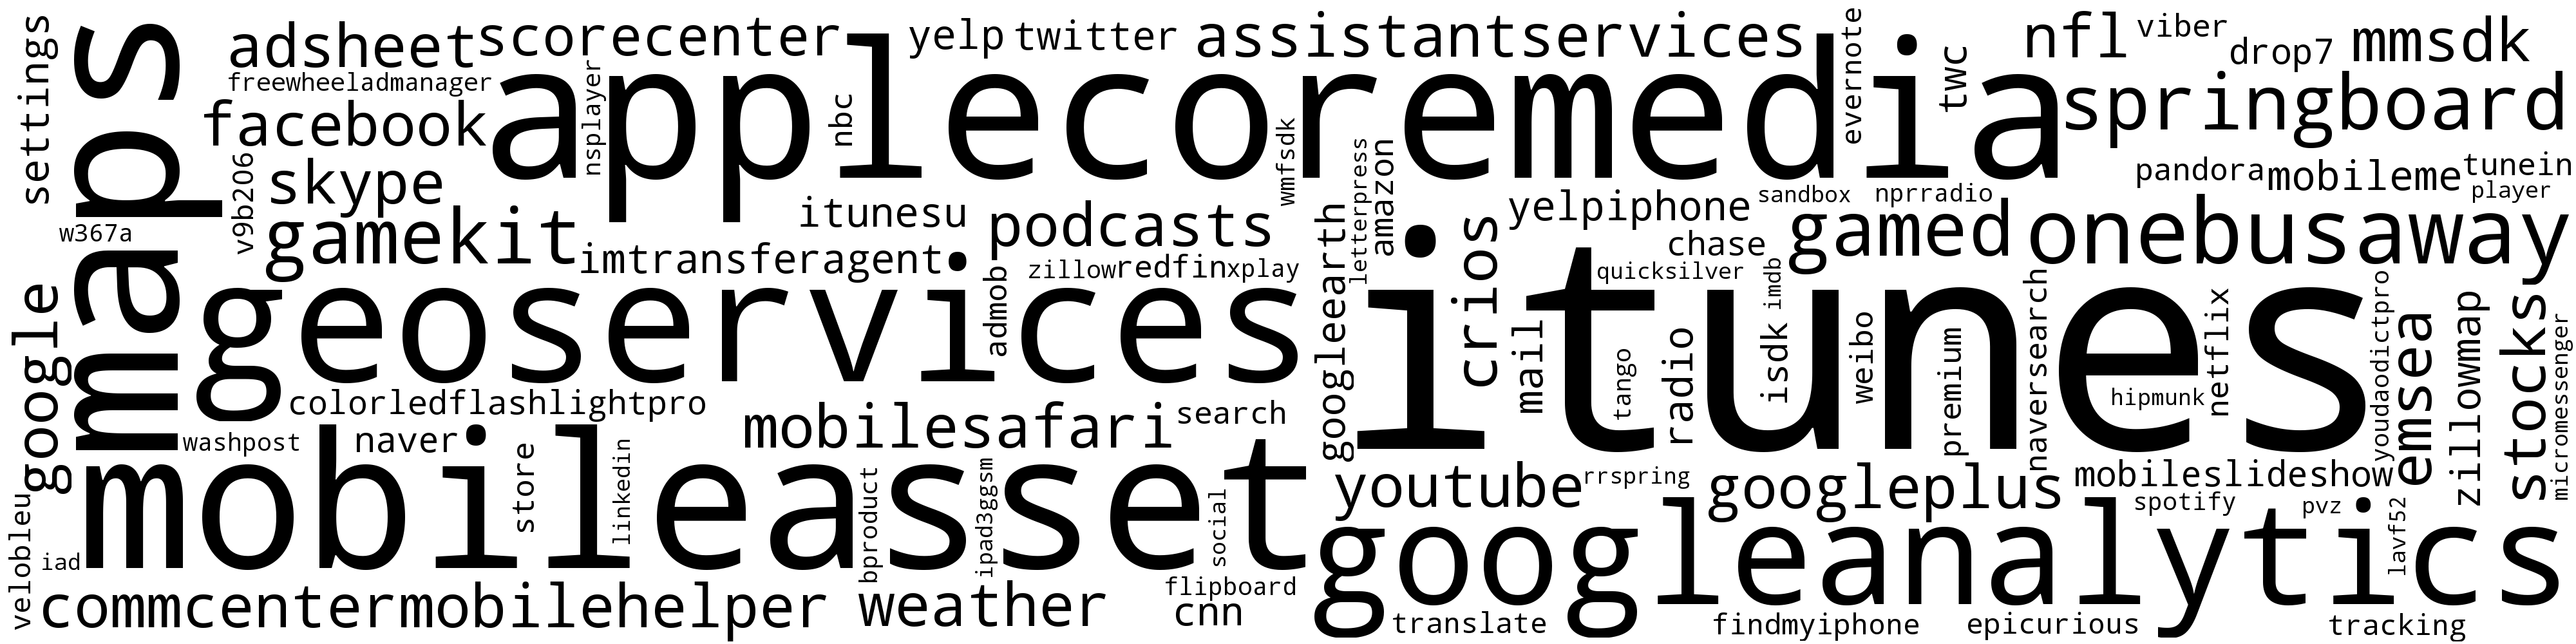
\includegraphics[width=\columnwidth]{figures/wordcloud_useragentsignature_ios_image.png}}\newline
\subfloat[Android]{\label{fig:http-wordcloud-android}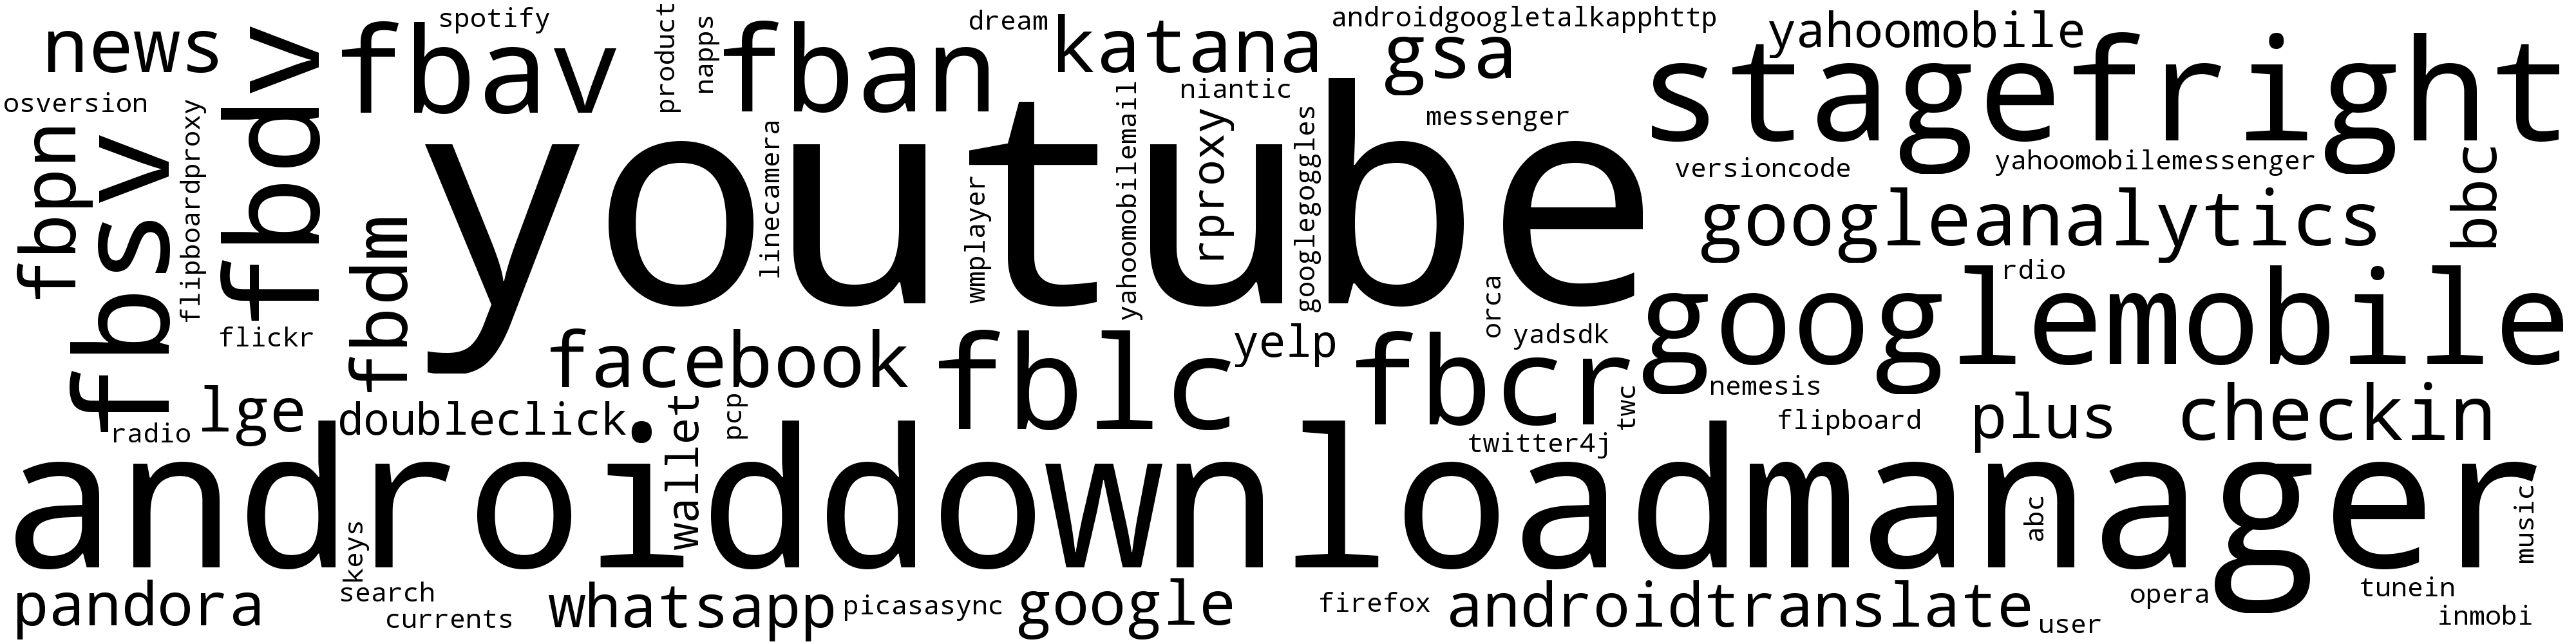
\includegraphics[width=\columnwidth]{figures/wordcloud_useragentsignature_android_image.png}}
\caption{\useragent signatures in  iOS and Android HTTP flows. \emph{The font weight represents the number of users for which a particular signature was observed.}}
\label{fig:http-wordcloud}
\end{figure}

On using this technique on the \mobWild dataset we were able to identify \tbd{} applications, which we summarize in \fref{fig:http-wordcloud}.
The \emph{word cloud} in \fref{fig:http-wordcloud} contains the signatures we were able to extract from \useragent field; the text size of the signature represents the number of users for which the signature was observed.
Along with signatures of applications such as iTunes and YouTube, we also observe signatures of the \emph{applecoremedia} and \emph{stagefright} services that are responsible to download media content on iOS and Android devices respectively.
Across the iOS and Android devices, we observe a total of \tbd{1435} unique \useragent strings that produce \tbd{361} unique signatures which we cluster to \tbd{} different applications and services. 


The use of OS services and media libraries to fetch media content resulted in the signature of AppleCoreMedia in more than 98.45\% of the content downloaded from the YouTube servers (which we identify based on the \httphost field in the \httpget requests). 
Similarly, depending the Android version we observe either the signature for Stagefright\cite{android:stagefright} or no application or OS service signature for YouTube traffic to Android devices depending on the OS version. 
For flows that used AppleCoreMedia, we observed signatures for popular media services such as Netflix, YouTube, Vimeo, Pandora, etc. in the \httphost field in the majority traffic. 

\begin{table}
\centering
\begin{small}
\begin{tabular}{|p{0.25\columnwidth}|c|c|c|c|}
\hline
\multirow{2}{*}{\bf Category} & \multicolumn{2}{c|}{\bf iOS} &  \multicolumn{2}{c|}{\bf Android} \tabularnewline
\cline{2-5}
  & {\bf Bytes}  & {\bf Flows} & {\bf Bytes} & {\bf Flows}   \tabularnewline
\hline
Media (Popular)         & 51.405  & 12.131 & 65.922 & 22.377 \tabularnewline
\hline
Application             & 33.987  & 80.758 & 31.353 & 77.498 \tabularnewline
\hline
Ads and Analytics       & \tbd{}  & \tbd{} & \tbd{}& \tbd{}\tabularnewline
\hline
Media (Other)           & 14.572  &  5.914 &  2.712 &  0.044 \tabularnewline
\hline
Other                   &  0.036  & 1.1963 &  0.013 &  0.081 \tabularnewline
\hline
{\em total}             & 100 & 100 & 100 & 100 \tabularnewline
\hline
\end{tabular}
\end{small}
\caption{Classification of HTTP Traffic. \emph{A total of \tbd{} iOS and \tbd{}Android applications were responsible for 80\% of iOS and 77\% of Android HTTP flows.}}
\label{tab:classify-http}
\end{table}

In \fref{tab:classify-http}, we observe that with a combination of \useragent and \httphost field in HTTP headers, we were able to classify more than 98\% of the traffic in terms of flows and bytes from iOS and Android devices.
We observe that media from popular hosts contribute to more than 50\% of the traffic volume from iOS and Android devices.
Similarly, we were able to identify applications for more than 77\% of flows from Android and iOS devices. 
However, we observe media (identified based on the \useragent) served from CDNs and others hosts from which we could not identify the webservice from other fields in the HTTP header and the DNS responses before the HTTP flows to be 14.5\% of the traffic volume for the iOS devices in our dataset.

\subsubsection{Classification of SSL Traffic.}

Unlike HTTP flows, SSL flows provide limited information that can be used to identify the applications. 
Our objective classifying SSL traffic was therefore focused towards identifying the Web-services responsible for the SSL flows. 
We now show how we used the port number, the SSL certificate with server name identification, and DNS queries to identify the source of SSL traffic. 

\begin{table}
\centering
\begin{small}
\begin{tabular}{|p{0.25\columnwidth}|c|c|c|c|}
\hline
\multirow{2}{*}{\bf Service} & \multicolumn{2}{c|}{\bf iOS} &  \multicolumn{2}{c|}{\bf Android} \tabularnewline
\cline{2-5}
  & {\bf Bytes}  & {\bf Flows} & {\bf Bytes} & {\bf Flows} \tabularnewline
\hline
HTTPS                   & 91.287 & 81.960 & 97.852 & 97.168    \tabularnewline
\hline
Mail                    &  6.700 & 15.872 & 0.689  & 0.320  \tabularnewline
\hline
Notification            &  1.412 & 1.553  & 1.321  & 2.100  \tabularnewline
\hline
Other                   &  0.601 & 0.615  & 0.138  & 0.412 \tabularnewline
\hline
{\em total}             & 100 & 100 & 100 & 100 \tabularnewline
\hline
\end{tabular}
\end{small}
\caption{Classification of SSL Traffic based on port number. \emph{HTTPs is the most popular service that uses SSL in the \mobWild dataset.}}
\label{tab:classify-ssl-port}
\end{table}

Mobile devices use SSL for various services including mail, notifications, instant messaging, and web browsing.
Services such as mail, instant messaging, and notifications are documented to use dedicated port numbers of their traffic\footnote{We also use the AS for identifying the notification messages as detailed in \fref{sec:characterize-os}.}
On using port numbers, we observe in \fref{tab:classify-ssl-port} that a majority of SSL traffic by volume and flows is HTTPS.
We then focus our attention on indentifying the Web-services responsible for the HTTPs flows. 

We first use the common name (CN) field of certificates to identify the servers that exchanged data using HTTPS.
We observe that less than 25\% of the HTTPS traffic from iOS and Android contains the fully qualified domain name (FQDN) in the subject of the certificate; the rest of the traffic either contains regular expressions such as *.google.com in the certificate or is a continuation of a previous SSL session. 
To further resolve the hostnames, we rely on \emph{server name indication} used by SSL flows~\cite{rfc:servernametls}.
Servers that host multiple services use the \emph{server name indication} to distinguish these services.   
For example, we observe a \emph{server name indication} of \emph{plus.google.com} and \emph{s.youtube.com} in two flows that used a certificate with a CN \emph{*.google.com}.
However, we observe that by using either the certificate or the \emph{server name} we were able to identify the name of the Web-service in less than \tbd{40}\% of iOS and Android HTTPS traffic.

For such flows we use DNS requests made by the mobile devices before starting the HTTPS flows, a technique similar to DN-Hunter~\cite{bermudez:dnhunter}.
DN-Hunter relies on the most recent FQDN that corresponds to the IP address, however in our controlled experiments we observe Android and iOS devices use the first entry in DNS response while resolving \emph{hostnames}.
We therefore use the latest DNS response that contains the IP address of the webservice in the first position of the DNS response. 
Indeed, for 97.8\% of the Android and 83.4\% of the iOS HTTPS traffic that we could not classify using other fields, we observe that the latest DNS response before the flow started contained the IP address of the webservice as the first entry in the DNS response\footnote{The share of SSL traffic where the latest DNS response contains the IP address of the web-service in the first position is 97.4\% for Android and 88.6\% of iOS}. 
Despite the potential usefulness of DNS responses, we give a high priority to the server-name and the certificates because we observed that for flows that contained the server name did not contain the same name in the DNS response for 9.2\% of the iOS traffic and 5.6\% of Android traffic.

\begin{table}
\centering
\begin{small}
\begin{tabular}{|c|c|}
\hline
{\bf iOS} & {\bf Android} \tabularnewline
\hline
imap.gmail.com & picasaweb.google.com \tabularnewline
www.google.com & www.googleapis.com \tabularnewline
sphotos-a.xx.fbcdn.net & android.clients.google.com \tabularnewline
itunes.apple.com  & clients4.google.com \tabularnewline
m.google.com & fbcdn-photos-a.akamaihd.net \tabularnewline
\hline
\end{tabular}
\end{small}
\caption{Popular hostnames for iOS and Android based on traffic volume.}
\label{tab:sslclassify-popular-host}
\end{table}

In \fref{tab:sslclassify-popular-host} we present the top5 hostnames that were responsible for 66\% of iOS traffic and 54\% of Android by volume. 
We observe that despite the hostname we cannot uniquely identify the application. 
For example, \emph{www.google-apis.com} and \emph{clients4.google.com} offer limited information on the application or web-service that is responsible for the content; one can only guess that these flows belong to some google service.
However, hostname such as \emph{fbcdn-photos-a.akamaihd.net} gives an indication that the traffic is due to facebook.

\begin{table}
\centering
\begin{small}
\begin{tabular}{|p{0.35\columnwidth}|c|c|c|c|}
\hline
\multirow{2}{*}{\bf Service} & \multicolumn{2}{c|}{\bf iOS} &  \multicolumn{2}{c|}{\bf Android} \tabularnewline
\cline{2-5}
  & {\bf Bytes}  & {\bf Flows} & {\bf Bytes} & {\bf Flows} \tabularnewline
\hline
Mail                 & 9.970    & 62.168   & 1.626  & 1.565 \tabularnewline
\hline
Social Networking    & 12.491   & 6.683    & 36.661 & 22.352 \tabularnewline
\hline
Apple/Google Store   & 5.457    & 3.463    & 0.044  & 0.036 \tabularnewline
\hline
Instant Messages     & 0.982    & 7.089    & 1.411  & 3.109 \tabularnewline
\hline
Other Google Services & 58.665   & 13.32510 & 45.024 & 46.089 \tabularnewline
\hline
\emph{total}         & 87.564   & 92.728   & 84.776 & 73.151 \tabularnewline
\hline
\end{tabular} 
\end{small}
\caption{Sample classification of SSL traffic based on names in certificate, server name identification, and DNS request.}
\label{tab:classify-ssl-traffic}
\end{table}

In \fref{tab:classify-ssl-traffic} we show how we grouped SSL traffic based on names identified using the SSL fields and DNS queries and port numbers.
We observe that the iOS devices in our dataset generated a significant number of flows to email sites.
Similarly, we were able to group 12.49\% of iOS and 36.661\% of Android traffic with social network services that includes \emph{Google Plus, Facebook, and Twitter}.
We speculate the increase in traffic share for Android devices is because Android devices offer services to backup photos on \emph{Google Plus}.
Similarly, we observe that 5.4\% of the traffic from iOS devices was from Apple stores while we observe only 0.04\% of traffic to the \emph{Google Play} store. 
This low share is because google can use hosts matching the pattern \emph{client*.google.com} to serve for different Web-services.
We observed a similar behavior in our controlled experiments, and we group such traffic as \emph{other google services}.
Indeed, in \fref{tab:classify-ssl-traffic} we observe that traffic from Google is the largest source of SSL traffic for iOS and Android devices in our dataset. 
\subsection{Case Study: Facebook Application in the Wild}

In summary, we use \platname to perform controlled experiments and in the wild measurements to characterize mobile Internet traffic. 
We use Bro to analyze the data and build on the output of bro to further classify HTTP flows and SSL flows to identify the source of the traffic. 
We now present the results of our experiments and measurements study. 


%%% Local Variables: 
%%% mode: latex
%%% TeX-master: "main.tex"
%%% End: 

% Popular webservices such as google are known to use the same pool of IP addresses for various applications, for example the IP for gmail may also be used for search. 
% In \fref{fig:ssl-classification-app-service} we present the fraction of SSL traffic where the most recent DNS response contained the IP address of the SSL flow in the first position. 
% We observe that for the majority of SSL traffic by volume and flows can be classified by using the DNS responses. 

% \begin{table}
% \centering
% \begin{small}
% \begin{tabular}{|p{0.35\columnwidth}|c|c|c|c|}
% \hline
% \multirow{2}{*}{\bf Service} & \multicolumn{2}{c|}{\bf iOS} &  \multicolumn{2}{c|}{\bf Android} \tabularnewline
% \cline{2-5}
%   & {\bf Bytes}  & {\bf Flows} & {\bf Bytes} & {\bf Flows} \tabularnewline
% \hline
% FQDN in Certificate    & 24.274 & 31.423  & 19.318 & 29.424 \tabularnewline
% \hline
% Regular expression     & 50.463 & 35.318  & 42.427 & 31.670 \tabularnewline
% \hline
% No Subject or CN       & 25.263 & 33.259  & 38.254 & 38.906 \tabularnewline
% \hline
% {\em total}            & 100 & 100 & 100 & 100 \tabularnewline
% \hline
% \end{tabular}
% \end{small}
% \caption{Classification of HTTPs based on certificates.}
% \label{tab:classify-http-cert}
% \end{table}

% We observe that more than 98\% of HTTP traffic from Android and iOS devices in the \mobWild dataset have a valid \useragent string; we observe a total of 1435 unique \useragent strings across Android and iOS devices. 
% These \useragent strings contain an application identifier and other auxiliary information such as details of the OS, manufacturer, display resolutions, carrier, and information such as versions and compatibility with other browser engines~\cite{mozilla:useragentdetection}. 
% We use regular expression to extract the tokens that contain the application information, and cluster these tokens using edit distance\footnote{We plan to release this code along with \platname package.}.
% At the end of this process we were able to identify 361 unique signatures which we resolve as either applications or OS services. 

% In \fref{fig:http-wordcloud} we present a \emph{word cloud} of the signatures we were able to extract from \useragent field; the text size of the signature represents the number of users for which the signature was observed.
% Despite the usefulness of the \useragent, we observe that relying only on the \useragent is not sufficient to identify the application.
% For example, we observe the signatures \emph{applecoremedia} and \emph{stagefright} in the \emph{word cloud} for iOS devices and Android devices, signatures of the OS services responsible to download media content.

% The iOS devices rely on AppleCoreMedia service~\cite{apple:coremedia} to download media content.
% We therefore observed the signature of AppleCoreMedia in more than 98.45\% of the content downloaded from the YouTube servers (which we identify based on the \httphost field in the \httpget requests). 
% Similarly, depending the Android version we observe either the signature for Stagefright\cite{android:stagefright} or no application or OS service signature for YouTube traffic to Android devices. 
% Indeed, we observed signatures for popular media services such as Netflix, YouTube, Vimeo, Pandora, etc. in the \httphost field in the majority traffic from iOS devices and Android devices. 
% We therefore used the \httphost field to classify media content.
